\section*{Experiment na reálném kameni}
Od počítačové simulace přejdeme k experimentu s reálným kamenem. Cílem experimentu je zjistit, zda výsledky, které naměříme lze porovnat s výsledky získanými pomocí matematického modelu. 

Zdrojem koherentního světelného svazku je laser. Laserové záření dopadá na broušený kámen, kde se roztříští na mnoho menších svazků. Svazky opouštějící kámen v horní polorovině jsou zachyceny na kulovém stínítku a na něm vznikne jedinečný světelný obrazec. Tento obrazec snímá kamera a vzniká digitální obraz. V obraze detekujeme laserové stopy na stínítku a z nich správnou transformací určujeme vlastnosti světelných svazků vystupujících z kamene. 

Zkoumaný kámen jsme vybrali ve tvaru šatonové růže s 12 bočními fasetami, tedy opět VIVA12 jako v počítačové simulaci. Jedná se o kámen červené barvy s označením Hyacint. Průměr kamene je takový, aby na celý jeho povrch dopadalo laserové záření. V našem případě \SI{2.8}{\milli\metre}. 
\begin{figure}[h!]
 \begin{center}
 

   \begin{minipage}[c]{0.69\textwidth}
     \centering \includegraphics[ height =5cm]{img/stolek} 
   \end{minipage}
   \begin{minipage}[c]{0.29\textwidth}
     \centering \includegraphics[height =5cm]{img/stolek-detail22} 
   \end{minipage}
 \end{center}

   \caption{Pohybová část měřicí soustavy. Laserové záření proniká otvorem na vrcholku bílé polokoule. Koherentní záření dopadá na kámen VIVA12 připevněný plastelínou na vrcholku prodloužení dvojice goniometrů. Goniometry je možné polohovat, kámen rotovat ve dvou osách a posouvat světelný obrazec po stínítku.}
   \label{fig:merici soustava}
 \end{figure}
 
 Kamenem jsme rotovali kolem tak, abychom mohli výsledky z reálného experimentu vizuálně porovnat s výsledky simulace. Při každém kroku jsme kámen rotovali o $\sqrt{2}$ stupně. Celkem jsme naměřili výsledky pro 41 pozic kaneme symetricky rozdělených kolem vrcholu půlkulového stínítka. Mezi obrazy lišícími se jedním krokem rotace jsme našli korespondující body. Při procesu hledání korespondencí vznikají chybná přiřazení. Je jich však tak málo, že při vizuálním porovnání nemají velký vliv. 
 
Korespondující body ze všech naměřených snímků jsme spojili do jednoho, přičemž jsme jejich pohyb znázornili vektory. Na obrázcích \ref{fig:graf posunu porovnani}, \ref{fig:relativni posun porovnani} je vidět porovnání výsledku se simulovanými daty.  

\begin{figure}[h!]
 \begin{center}
 

   \begin{minipage}[c]{0.49\textwidth}
     \centering 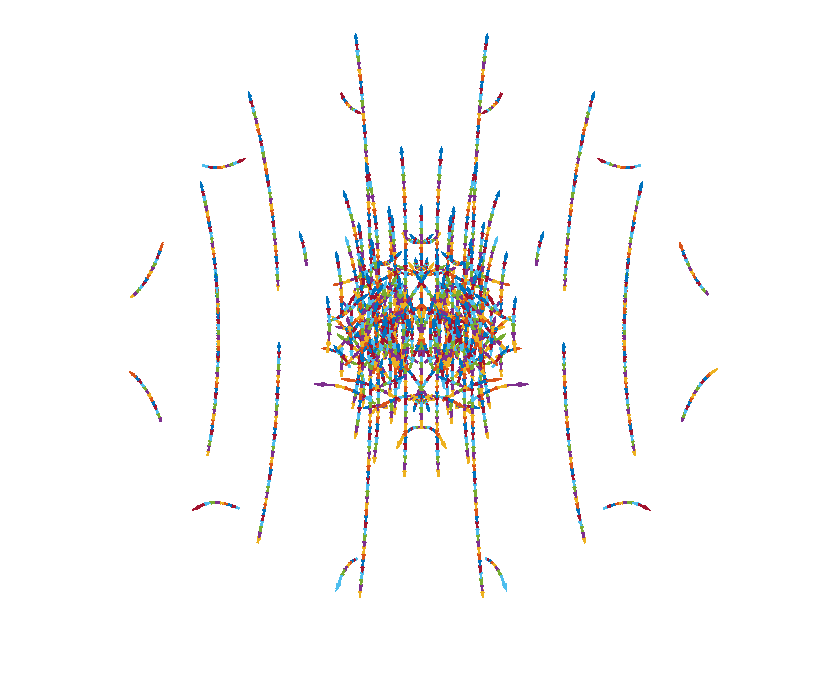
\includegraphics[height =5cm]{figures/viva12_bigflux} 
   \end{minipage}
   \begin{minipage}[c]{0.49\textwidth}
     \centering 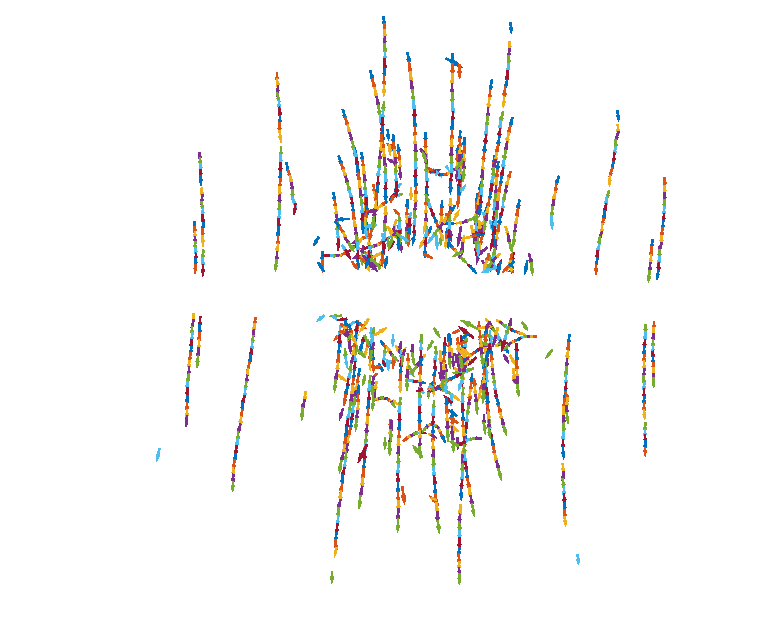
\includegraphics[height =5cm]{figures/real_all} 
   \end{minipage}
 \end{center}

   \caption{Porovnání výsledku z počítačové simulace s výsledky z reálného experimentu. Vlevo máme výsledky posunu stop kamene  vypočtené pomocí matematického modelu kamene. Obrázek je totožný s obr. \ref{fig:relativni pohyb graf}. Obrázek vpravo znázorňuje výsledky z experimentu s reálným kamenem. Data nejsou úplná, neboť z pohledu kamery část půlkulového stínítka zakrývá konstrukce pro připevnění goniometrů. Oba výsledky jsou si vizuálně podobné. Blízko středu obrázku se objevují typické oblouky spojené se svazky podobného typu, jako na obrázku \ref{fig:odrazy v kamenu}, kde je znázorněna jeho trasa kamenem.}
   \label{fig:graf posunu porovnani}
 \end{figure}
 
\begin{figure}[h!]
 \begin{center}
 

   \begin{minipage}[c]{0.45\textwidth}
     \centering 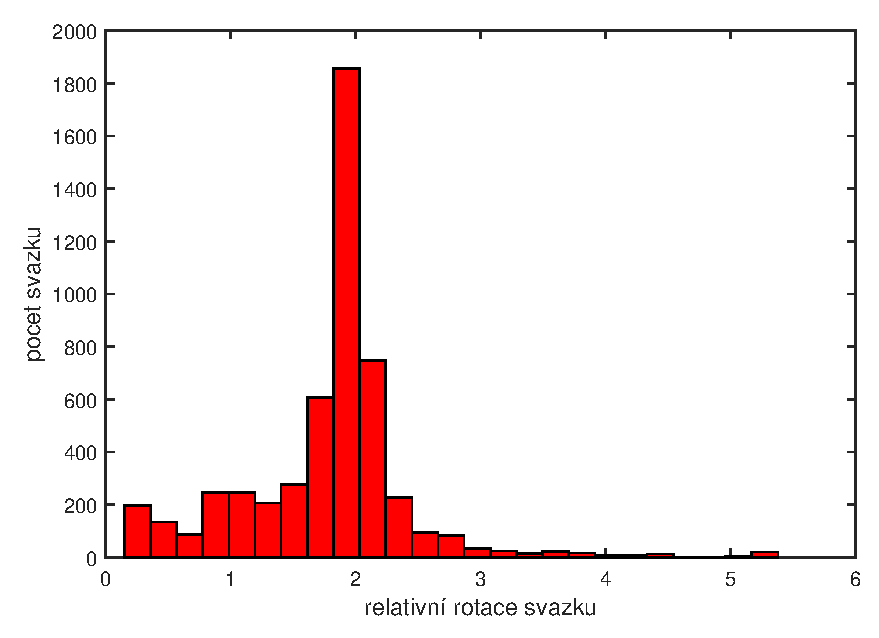
\includegraphics[height =4.5cm]{figures/relative} 
   \end{minipage}
   \begin{minipage}[c]{0.45\textwidth}
     \centering 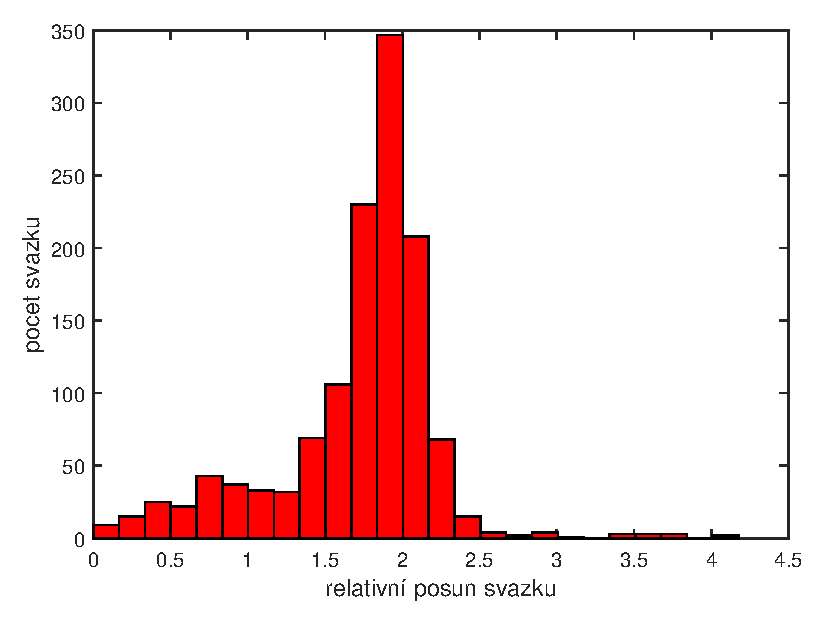
\includegraphics[height =4.5cm]{figures/real_relative} 
   \end{minipage}
 \end{center}

   \caption{Porovnání výsledku z počítačové simulace s výsledky z reálného experimentu - velikost posunu. Vlevo máme histogram velikosti posunu stop kamene  vypočtené pomocí matematického modelu kamene. Obrázek je totožný s obr. \ref{fig:histogram relativni pohyb } vlevo. Obrázek vpravo znázorňuje histogram velikosti posunu stop z experimentu s reálným kamenem. Podobnost je i zde patrná.}
  \label{fig:relativni posun porovnani}
 \end{figure}